\section{Resultados}
	\begin{frame}
		\begin{center}
			\begin{huge}
				{Resultados}
			\end{huge}
		\end{center}
	\end{frame}
	\subsection{Baselines}
		\begin{frame}
				\frametitle{Parámetros iniciales}
				\textit{Parámetros iniciales con el que se corrió el primer experimento}
				\begin{itemize}
					\item<1-> \textit{Cantidad de grupos:} \textbf{256}
					\item<2-> \textit{Bits por grupo:} \textbf{6}
					\item<3-> \textit{Método de umbralización:} \textbf{Generación de variables aleatorias uniformes}
					\item<4-> $\alpha$: $\{0.01, 0.1, 1\}$
					\item<5-> \textit{HOG:}
						\begin{itemize}
							\item<6-> \textit{Orientaciones:} $\{8, 9\}$
							\item<7-> \textit{Celdas por bloque:} $\{4, 9\}$
						\end{itemize}
				\end{itemize}
		\end{frame}
		\begin{frame}
				\frametitle{Resultados del primer experimento}
				\begin{table}
				\centering
	    				\begin{tabular}{ | l | l | l | p{5cm} |}
    						\hline
    						\textbf{Implementación} & \textbf{Score} \\ \hline
    						Wang NATIVE+FERNS & 54\% \\ \hline
    						Impl. propia NATIVE+FERNS & 50\% \\ \hline
    						Wang SYNTH+FERNS & 47\% \\ \hline
    						Impl. propia SYNTH+FERNS & 43\% \\
   						\hline
    					\end{tabular}
				\end{table}
				\pause
				Se eligen los siguientes parámetros para el resto de los experimentos:
				\begin{itemize}
					\item<1-> HOG:
						\begin{itemize}
							\item<2-> \textit{Orientaciones:} \textbf{8}
							\item<3-> \textit{Celdas por bloque:} \textbf{9}
						\end{itemize}
					\item<4-> $\alpha$: \textbf{0.01}						 				
				\end{itemize}
		\end{frame}
	\subsection{Resultados esquemas de binarizacion}
		\begin{frame}
			\frametitle{Esquema de binarización: \textit{Media}}
			\begin{figure}[htbp!]
				\centering
				\centerline{
					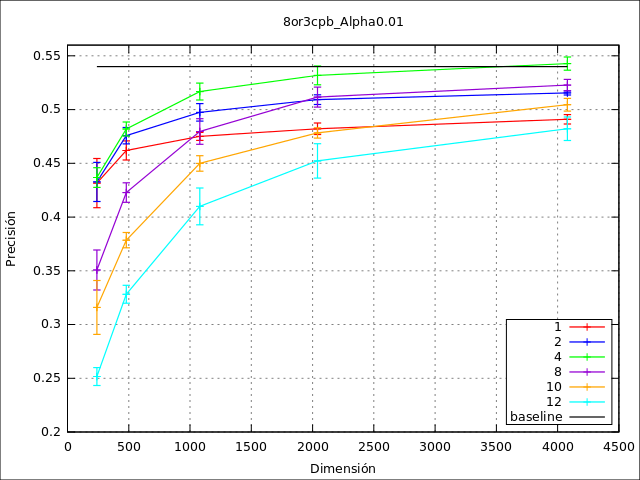
\includegraphics[height=0.65\paperheight]{../img/resultados/reales/mean.png}
				}
			\end{figure}
		\end{frame}
		\begin{frame}
			\frametitle{Esquema de binarización: \textit{Mediana}}
			\begin{figure}[htbp!]
				\centering
				\centerline{
					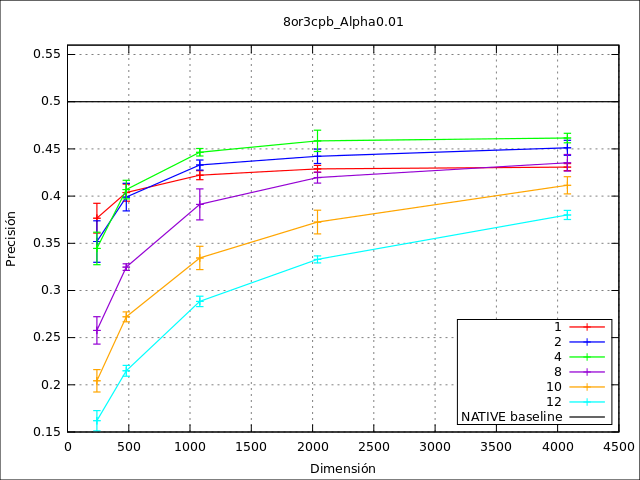
\includegraphics[height=0.65\paperheight]{../img/resultados/reales/median.png}
				}
			\end{figure}
		\end{frame}
		\begin{frame}
			\frametitle{Esquema de binarización: \textit{Bootstrap}}
			\begin{figure}[htbp!]
				\centering
				\centerline{
					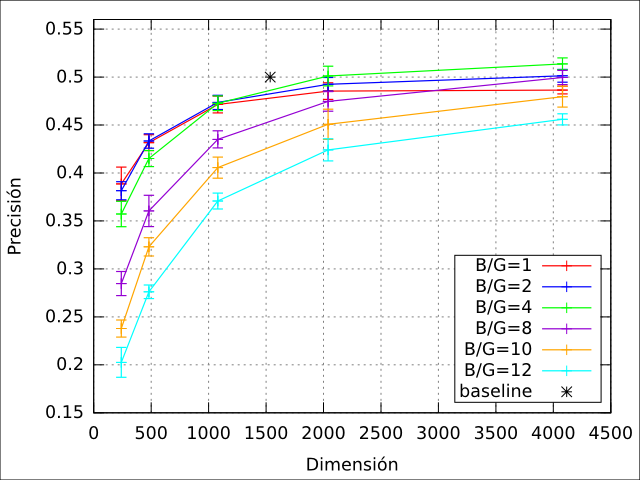
\includegraphics[height=0.65\paperheight]{../img/resultados/reales/bootstrap.png}
				}
			\end{figure}
		\end{frame}
		\begin{frame}
			\frametitle{Esquema de binarización: \textit{Exponencial}}
			\begin{figure}[htbp!]
				\centering
				\centerline{
					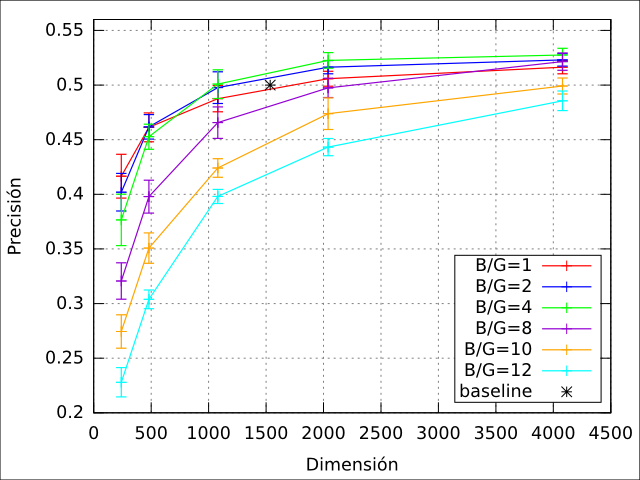
\includegraphics[height=0.65\paperheight]{../img/resultados/reales/expon.png}
				}
			\end{figure}
		\end{frame}
		\begin{frame}
			La mejor configuración obtenida se da con los siguientes parámetros:
			\begin{itemize}
				\item<1-> \textit{Bits por grupo:}~\textbf{4}
				\item<2-> \textit{Dimensión del vector:}~\textbf{2040}
			\end{itemize}
		\end{frame}
		\begin{frame}
			\frametitle{Mejor curva para cada esquema}
			\begin{figure}[htbp!]
				\centering
				\centerline{
					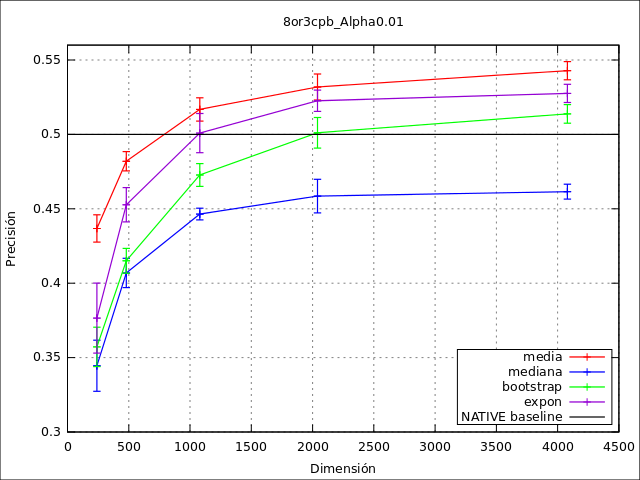
\includegraphics[height=0.60\paperheight]{../img/resultados/reales/comparativa_metodos.png}
				}
			\end{figure}
			\begin{itemize}
				\centering
				\item<1-> Mejor esquema de binarización:~\textit{Media}.
			\end{itemize}
		\end{frame}
	\subsection{Resultados imagenes sinteticas}
		\begin{frame}
			\frametitle{Conjunto sintético}
			\begin{figure}[htbp!]
				\centering
				\centerline{
					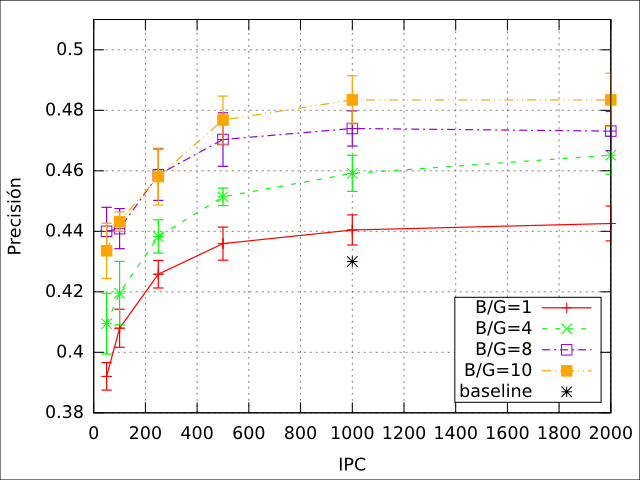
\includegraphics[height=0.65\paperheight]{../img/resultados/sinteticas/mean_2040.png}
				}
			\end{figure}
		\end{frame}
		\begin{frame}
			\frametitle{Conjunto mixto}
			\begin{figure}[htbp!]
				\centering
				\centerline{
					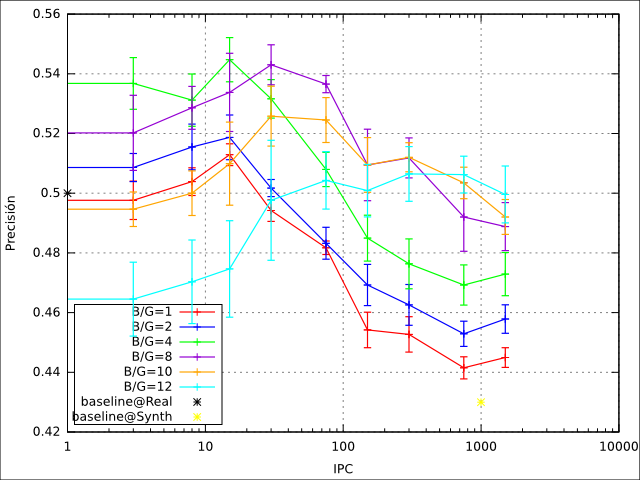
\includegraphics[height=0.65\paperheight]{../img/resultados/mixtas/best_mean_2040.png}
				}
			\end{figure}
		\end{frame}
		\begin{frame}
			\frametitle{Errores de clasificación}
			\begin{itemize}
				\item Confundir un caracter por otro similar.
			\end{itemize}
			\begin{figure}[htbp!]
				\centering
				\centerline{
					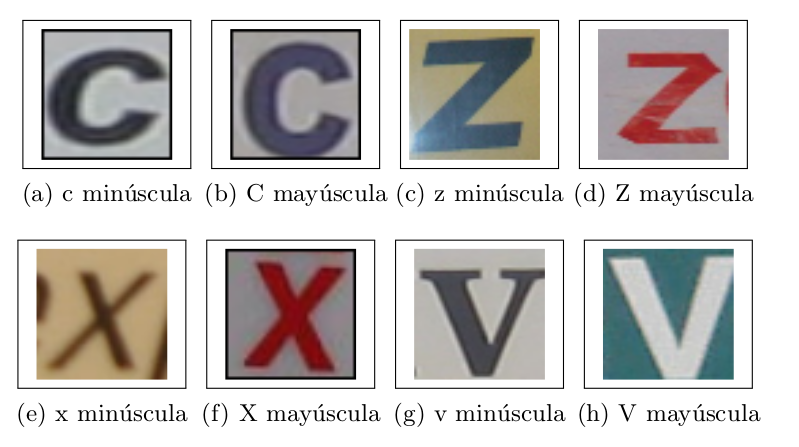
\includegraphics[height=0.50\paperheight]{imgs/error_may_min.png}
				}
			\end{figure}
		\end{frame}
		\begin{frame}
			\frametitle{Errores de clasificación}
			\begin{itemize}
				\item No poder distinguir mayúsculas de minúsculas para los caracteres involucrados.
			\end{itemize}
			\begin{figure}[htbp!]
				\centering
				\centerline{
					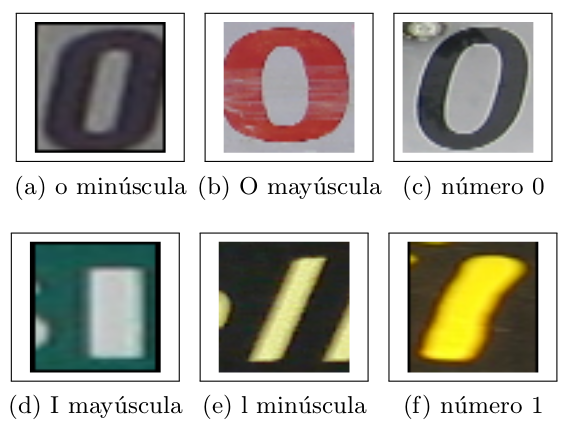
\includegraphics[height=0.50\paperheight]{imgs/error_conf_simbolos.png}
				}
			\end{figure}
		\end{frame}
		\begin{frame}
			\frametitle{Matriz de confusión}
			\includegraphics<1>[height=0.75\paperheight]{../img/resultados/mixtas/best_mean_matrix_Alpha0,01_2040-4.png}
			\includegraphics<2>[height=0.75\paperheight]{imgs/matriz_conf_diagonal_principal.png}
			\includegraphics<3>[height=0.75\paperheight]{imgs/matriz_conf_diagonal_secundaria.png}
			\includegraphics<4>[height=0.75\paperheight]{imgs/matriz_conf_confusion_simb.png}

		\end{frame}
		\begin{frame}
			\frametitle{Matriz de confusión \textit{case insensitive}}
			\begin{figure}[htbp!]
				\centering
				\centerline{
					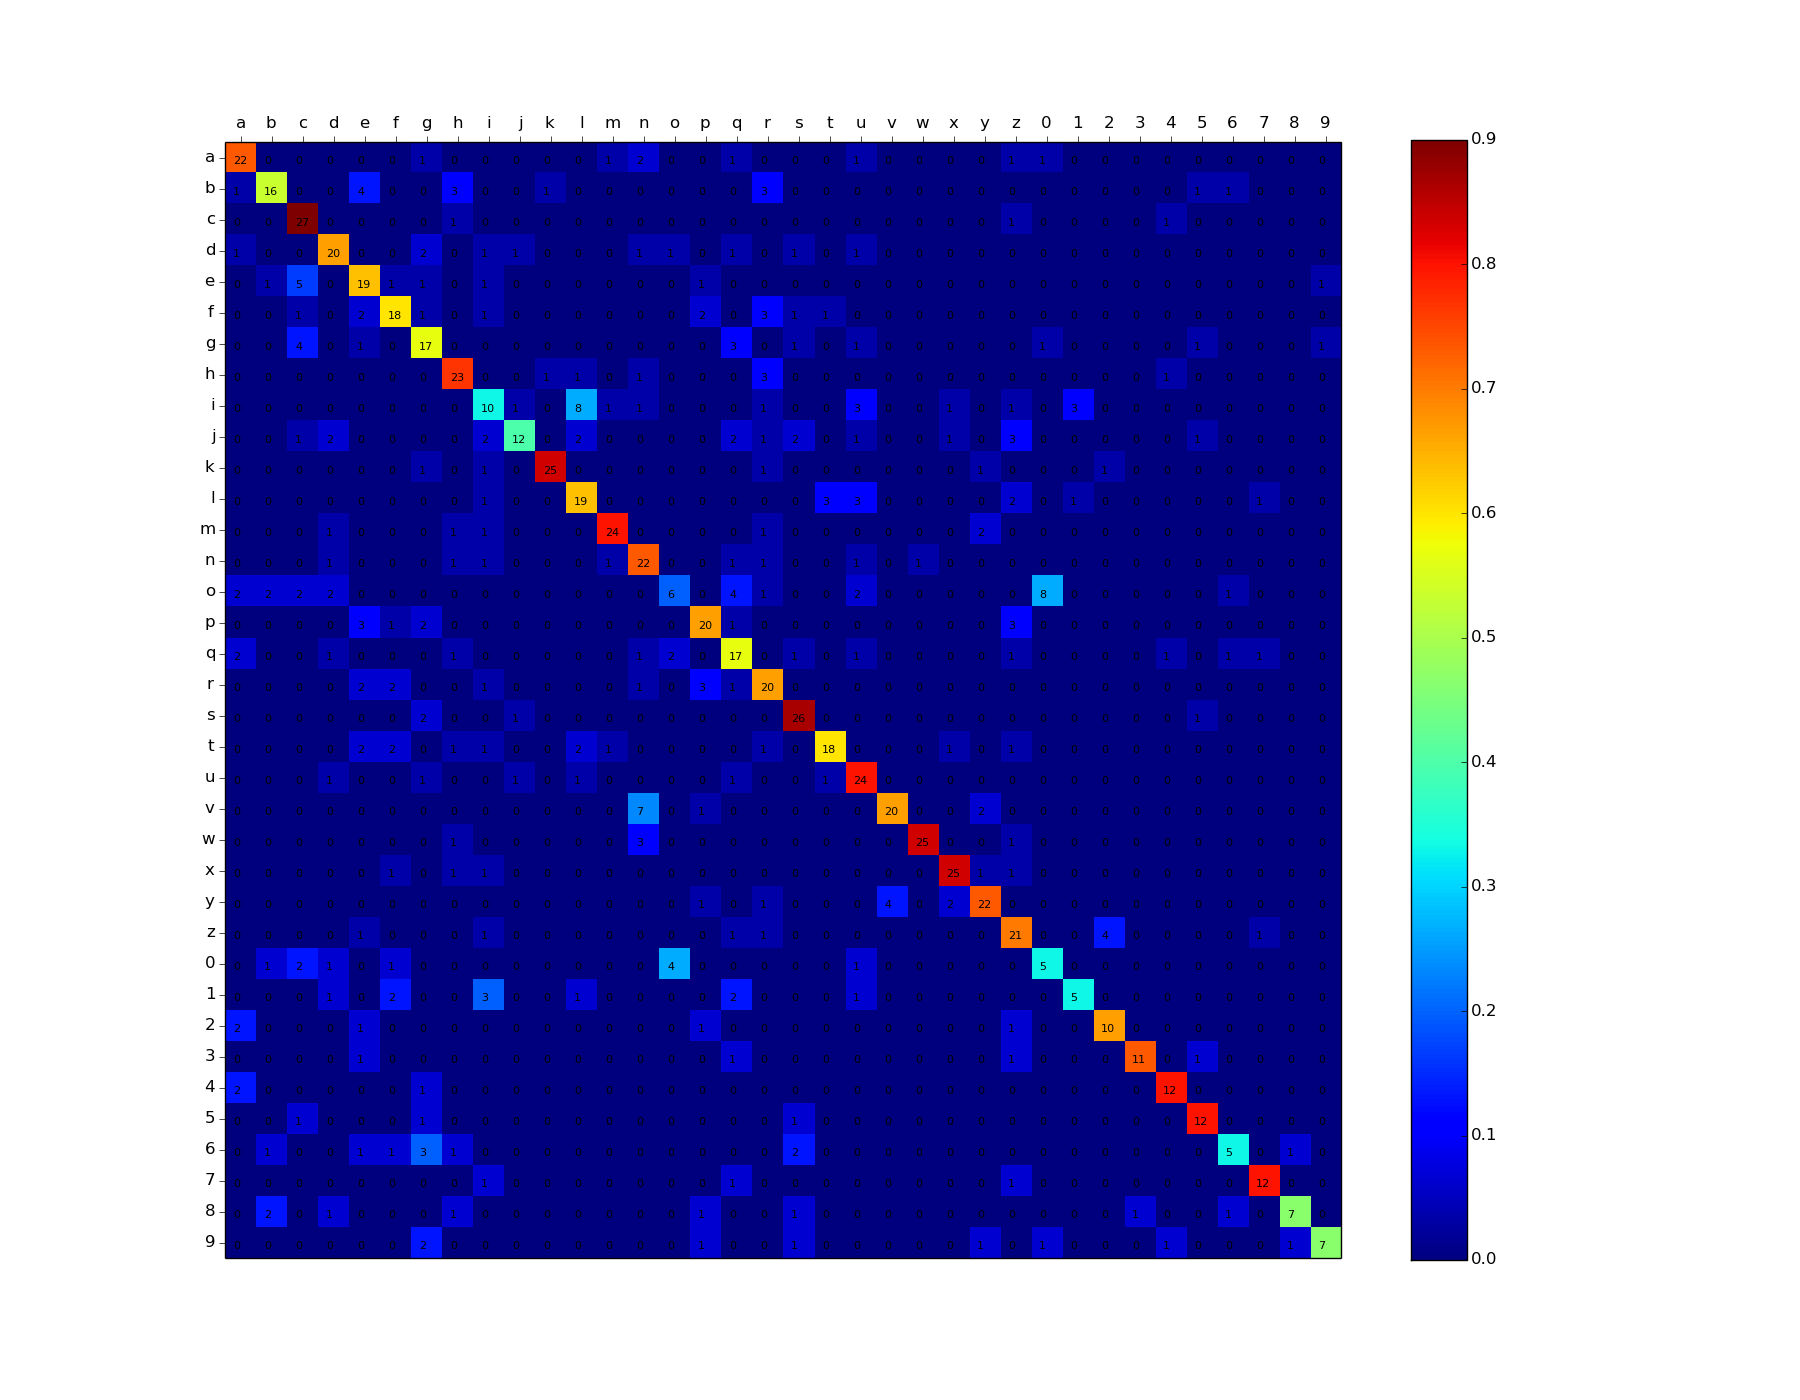
\includegraphics[height=0.75\paperheight]{../img/resultados/mixtas/best_mean_matrix_Alpha0,01_2040-4_ins.png}
				}
			\end{figure}
		\end{frame}